\IfFileExists{../../_preamble/check_file.tex}% prüfen aus welcher datei der aufruf stattfindet
{%
\providecommand{\myPath}{../../}% file exists=true: befinde mich im unterverzeichnis
}%
{%
\providecommand{\myPath}{}% file exists=false: befinde mich im root_verzeichnis
}%
\documentclass[tikz]{standalone}
%% läd standalone-klasse mit tikz-argument
%//Tikzbibliotheken\\%
\usetikzlibrary{						% Bibliotheken zur direkten Einbindung in TIKZEdt
arrows, 
fit,
shapes.geometric, 
matrix,
calc,
decorations.markings,
decorations.pathreplacing,
decorations.pathmorphing,
backgrounds,
shadings, 
shadows,
positioning,
mindmap,
trees,
datavisualization
}%% diverse tikz-bibliotheken
%%Font etc.%%
\usepackage{lmodern}					% OK, Latin Modern font,											check: 25.08.18
\usepackage{xcolor} 					% OK, Definieren und Nutzen von versch. Farben						check: 25.08.18
\usepackage{graphicx}					% OK, Bereitstellen von \includegraphics							check: 25.08.18

%%Forest%%
\usepackage{forest}						% OK, Baumdarstellung aus dem linguistischen Bereich				check: 25.08.18
\useforestlibrary{edges}

%%Venndiagramm%%
\usepackage{venndiagram}				% OK, Definieren und Darstellen von Venndiagrammen					check: 25.08.18

%%Tabellen%%
\usepackage{booktabs}					% OK, Schönere Tabellen ohne vertikale Linien \toprule etc.			check: 25.08.18
\usepackage{tabularx}					% OK, Weiterer Spaltentyp passt Tabellenbreite  automatisch an		check: 25.08.18
\usepackage{multirow}					% OK, Zellenspannung über mehrere Zeilen							check: 25.08.18
%\usepackage{makecell}					% OK, Tabellenlayout (Tabaellenheader) ähnlich \multirow			check: 25.08.18
\usepackage{tablefootnote}				% OK, Fußnoten in Tabellen (\footnote funktioniert nicht)			check: 25.08.18
\usepackage{array} 						% OK, Erstellen eigener Columntypen in Tabellenumgebungen			check: 25.08.18

%%Grafiken und Plots%%
\usepackage{tikz} 						% OK, Natives zeichnen in Latex ,									check: 25.08.18
\usepackage{tikz-cd} 					% OK, Erstellen von kommutativen Diagrammen in Tikz,				check: 25.08.18
\usepackage{pgfplots}					% OK, Plotten von Daten,											check: 25.08.18
\pgfplotsset{compat=newest}				% OK, Einstellen der Kompatibilitätsversion,						check: 25.08.18
\usepackage{pgfplotstable}				% OK, Plotten und schreiben von Daten in Tabellen,					check: 25.08.18
\usepackage{pgfcalendar} 				% OK, Umrechnen von Datumskoordinaten,								check: 25.08.18
\usepgfplotslibrary{dateplot}			% OK, Plotten von Datumskoordinaten,								check: 25.08.18
\usepgfplotslibrary{units}				% OK, Darstellen von Einheiten als Achsenlabel,						check: 25.08.18%% nur laden wenn weitere graphic pakete benötigt werden (tabellen, pgfplot,...)
%%define tikz-stlyes here, colours etc.
\tikzset{
block_phantom/.style={block_normal, draw=red, fill=none},
block_phantom/.style={block_normal, draw=blue, fill=none}
}
%\tikzstyle{block_phantom}=[block_normal, draw=red, fill=none]%% tikz-styles, farben etc.
\begin{document}%
\IfFileExists{../../_preamble/check_file.tex}% prüfen aus welcher datei der aufruf stattfindet
{%file exists=true: befinde mich im unterverzeichnis
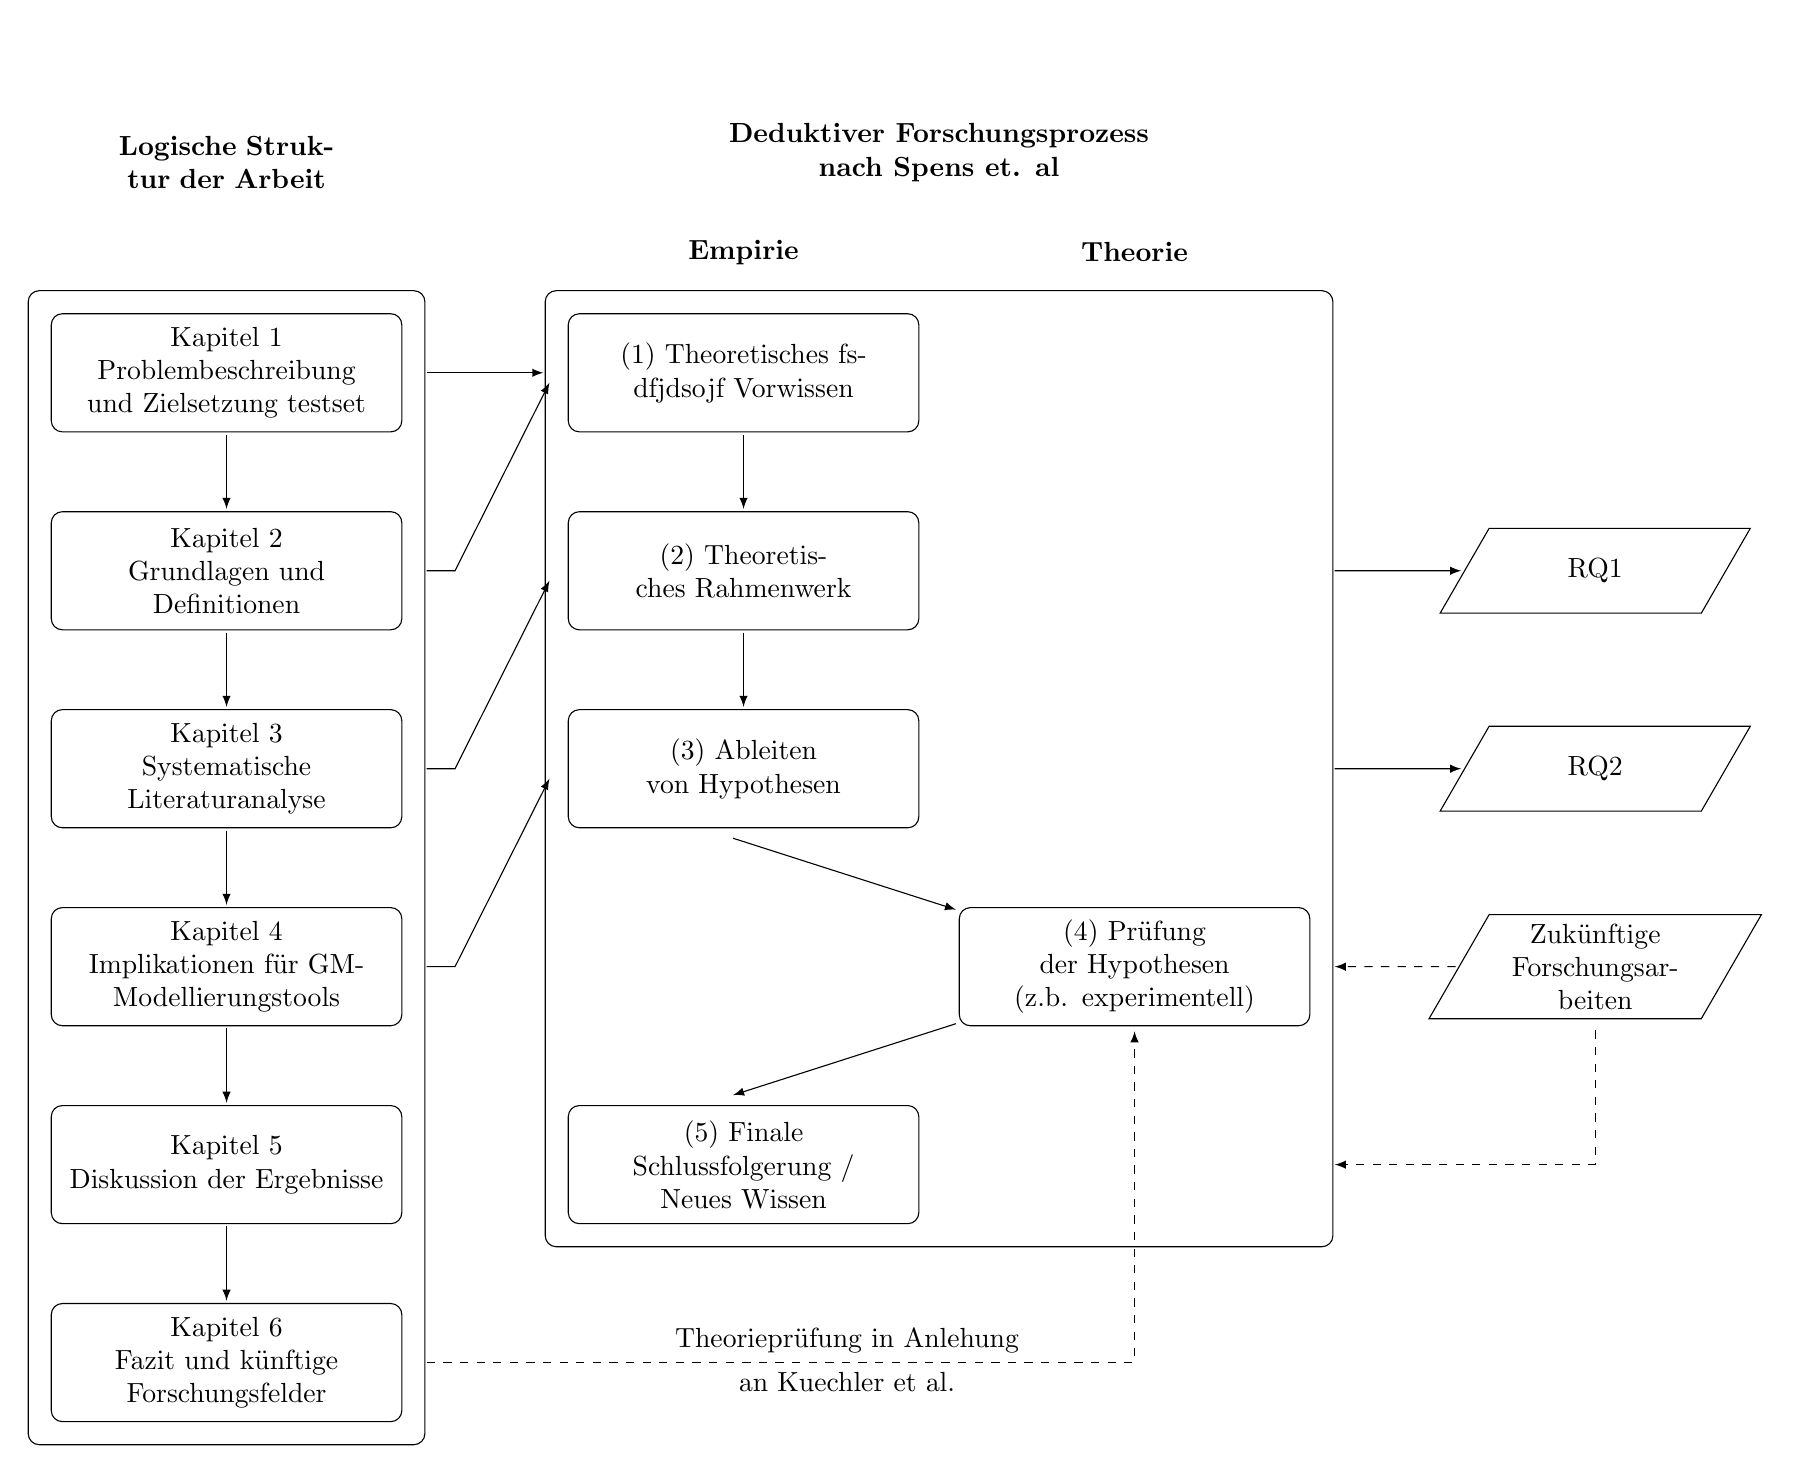
\begin{tikzpicture}
[auto, 
decision/.style={diamond, draw=blue, thick, fill=blue!20,text width=4.5em,align=flush center,inner sep=1pt},
block/.style ={ rectangle, draw, fill=white,  text centered, minimum height=15mm, text width=12em},
block_todo/.style ={ rectangle, draw, fill=white,  text centered, minimum height=15mm, text width=12em, rounded corners, outer sep=5},
block_done/.style ={ rectangle, draw, fill=white,  text centered, minimum height=15mm, text width=12em, rounded corners, outer sep=5},
block_normal/.style ={ rectangle, draw, fill=white,  text centered, minimum height=15mm, text width=12em, rounded corners, outer sep=5},
block_phantom/.style ={ block_normal, draw=none},
block_background/.style ={ rectangle,  draw=, fill=none,  text centered, minimum height=15mm,fill opacity=.1, rounded corners},
output/.style ={trapezium,draw,fill=none, minimum height=10mm,  align=center, trapezium left angle=60, trapezium right angle=120, text width=70},
line_inner/.style ={draw, -latex,shorten >=-4pt, shorten <=-4pt},
line_outer/.style ={draw, -latex,shorten >=4pt, shorten <=4pt}]
]


\matrix (table) [column sep=1.5cm,row sep=1cm, ampersand replacement=\&,  nodes in empty cells, in front of path]
{
% row 1
\node [block_normal, draw=none] (11) {\textbf{Logische Struktur der Arbeit}};\& [.6cm]
 \node [block_normal, fill=none, draw=none] (12) {\\ \quad\\\quad\\\quad\\\quad\\\quad\\\textbf{Empirie}}; \&[-1cm]
 \node [block_normal, fill=none, draw=none] (13) {\\ \quad\\\quad\\\quad\\\quad\\\quad\\\textbf{Theorie}};  \& [0cm]
 \node [] (14) {};   \\[-.5cm]

% row 2
\node [block_normal] (21) {Kapitel 1\\Problembeschreibung und Zielsetzung testset};
\&  \node [block_done] (22) {(1) Theoretisches fsdfjdsojf Vorwissen};
\&  \node [block_phantom] (23) {};
\&  \node [] (24) {};
\\

% row 3
\node [block_normal] (31) {Kapitel 2\\Grundlagen und Definitionen}; \& 
\node [block_done] (32) {(2) Theoretisches Rahmenwerk};  
\&\node [block_phantom] (33) {};  ;
\& \node [output] (34) {RQ1\vphantom{\begin{tabular}{c}x\\ y\end{tabular}}};
\\
% row 4
\node [block_normal] (41) {Kapitel 3\\Systematische Literaturanalyse}; \&
\node [block_done] (42) {(3) Ableiten von Hypothesen}; \&   
\node [block_phantom] (43) {}; 
 \&\node [output] (44) {RQ2\vphantom{\begin{tabular}{c}x\\ y\end{tabular}}};\\
 
% row 5
\node [block_normal] (51) {Kapitel 4\\Implikationen f\"ur GM-Modellierungstools}; \& 
\node [block_phantom] (52) {}; \&  
\node [block_done] (53) {(4) Pr\"ufung der Hypothesen\\ (z.b. experimentell)};
 \&\node [output] (54) {Zuk\"unftige Forschungsarbeiten}; \\

% row 6
\node [block_normal] (61) {Kapitel 5\\Diskussion der Ergebnisse};\& 
\node [block_done] (62) {(5) Finale Schlussfolgerung / \\Neues Wissen};
 \& \node [block_phantom] (63) {};
 \&  \node [] (64) {};\\
 
% row 7
\node [block_normal] (71) {Kapitel 6\\Fazit und k\"unftige Forschungsfelder}; \& 
\node [block, fill=none, draw=none] (72) {};  \&  
\node [block, fill=none, draw=none] (73) {};\&  
\node [] (74) {};\\
};


\begin{scope}[on background layer]
%%%HEADER%%%%%
\node[fit=(12)(13), draw=none, minimum height=1cm, fill=none]{\textbf{Deduktiver Forschungsprozess\\ nach Spens et. al}};
%%%%%SPALTE1%%%%%%%%%
\node[fit=(21)(71), block_background, fill=white]{};
%%%%%SPALTE2%%%%%%%%
\node[fit=(22)(63), block_background]{};
\end{scope}
 
 
%Pfeile Kapitelstruktur
 \draw [line_inner](21) to [bend left=0] node [above] {} (31)  ;
 \draw [line_inner](31) to [bend left=0] node [above] {} (41)  ;
 \draw [line_inner](41) to [bend left=0] node [above] {} (51)  ;
 \draw [line_inner](51) to [bend left=0] node [above] {} (61)  ;
 \draw [line_inner](61) to [bend left=0] node [above] {} (71)  ;


%Pfeile Prozess
 \draw [line_inner](22) to [bend left=0] node [above] {} (32);
 \draw [line_inner](32) to [bend left=0] node [above] {} (42)  ;
 \draw [line_inner](42.south) to [bend left=0] node [above] {} (53)  ;
 \draw [line_inner](53) to [bend left=0] node [above] {} (62.north)  ;

%Pfeile Interaktion Kapitel Prozess
 \draw [line_outer](21.east) to [bend left=0] node [above] {} (22.west)  ;
% \draw [line_outer](31.east) to [bend left=0] node [above] {$$} (22.west)  ;
  \draw [line_outer](31.east) -| ++ (.5,0) --  node [above] {} (22.west)  ;
% \draw [line_outer](41.east) to [bend left=0] node [above] {$$} (32.west)  ;
 \draw [line_outer](41.east) -| ++ (.5,0) --  node [above] {} (32.west)  ;
 %\draw [line_outer](51.east) to [bend left=0] node [above] {$$} (42.west)  ;
  \draw [line_outer](51.east) -| ++ (.5,0) --  node [above] {} (42.west)  ;
 %\draw [line](61) to [bend left=0] node [above] {$$} (22)  ;
% \draw [line](71.east) to [bend right=40] node [above] {$$} (53)  ;
 \draw [line_outer, dashed,shorten >=-3pt](71.east) -|   node [above, pos=.3] {Theoriepr\"ufung in Anlehung }  node [below, pos=.3] {an Kuechler et al.}(53)  ;
 
%Pfeile Output
 \draw [line_outer, shorten >=1pt](33) to [bend left=0] node [above] {} (34)  ;
 \draw [line_outer,shorten >=1pt](43) to [bend left=0] node [above] {} (44)  ;
 \draw [line_outer, dashed,shorten <=1pt](54) to [bend left=0] node [above] {} (53)  ;
  \draw [line_outer, dashed](54) |-  node [above] {} (63)  ;

\end{tikzpicture}%
}%
{%file exists=false: befinde mich im root_verzeichnis
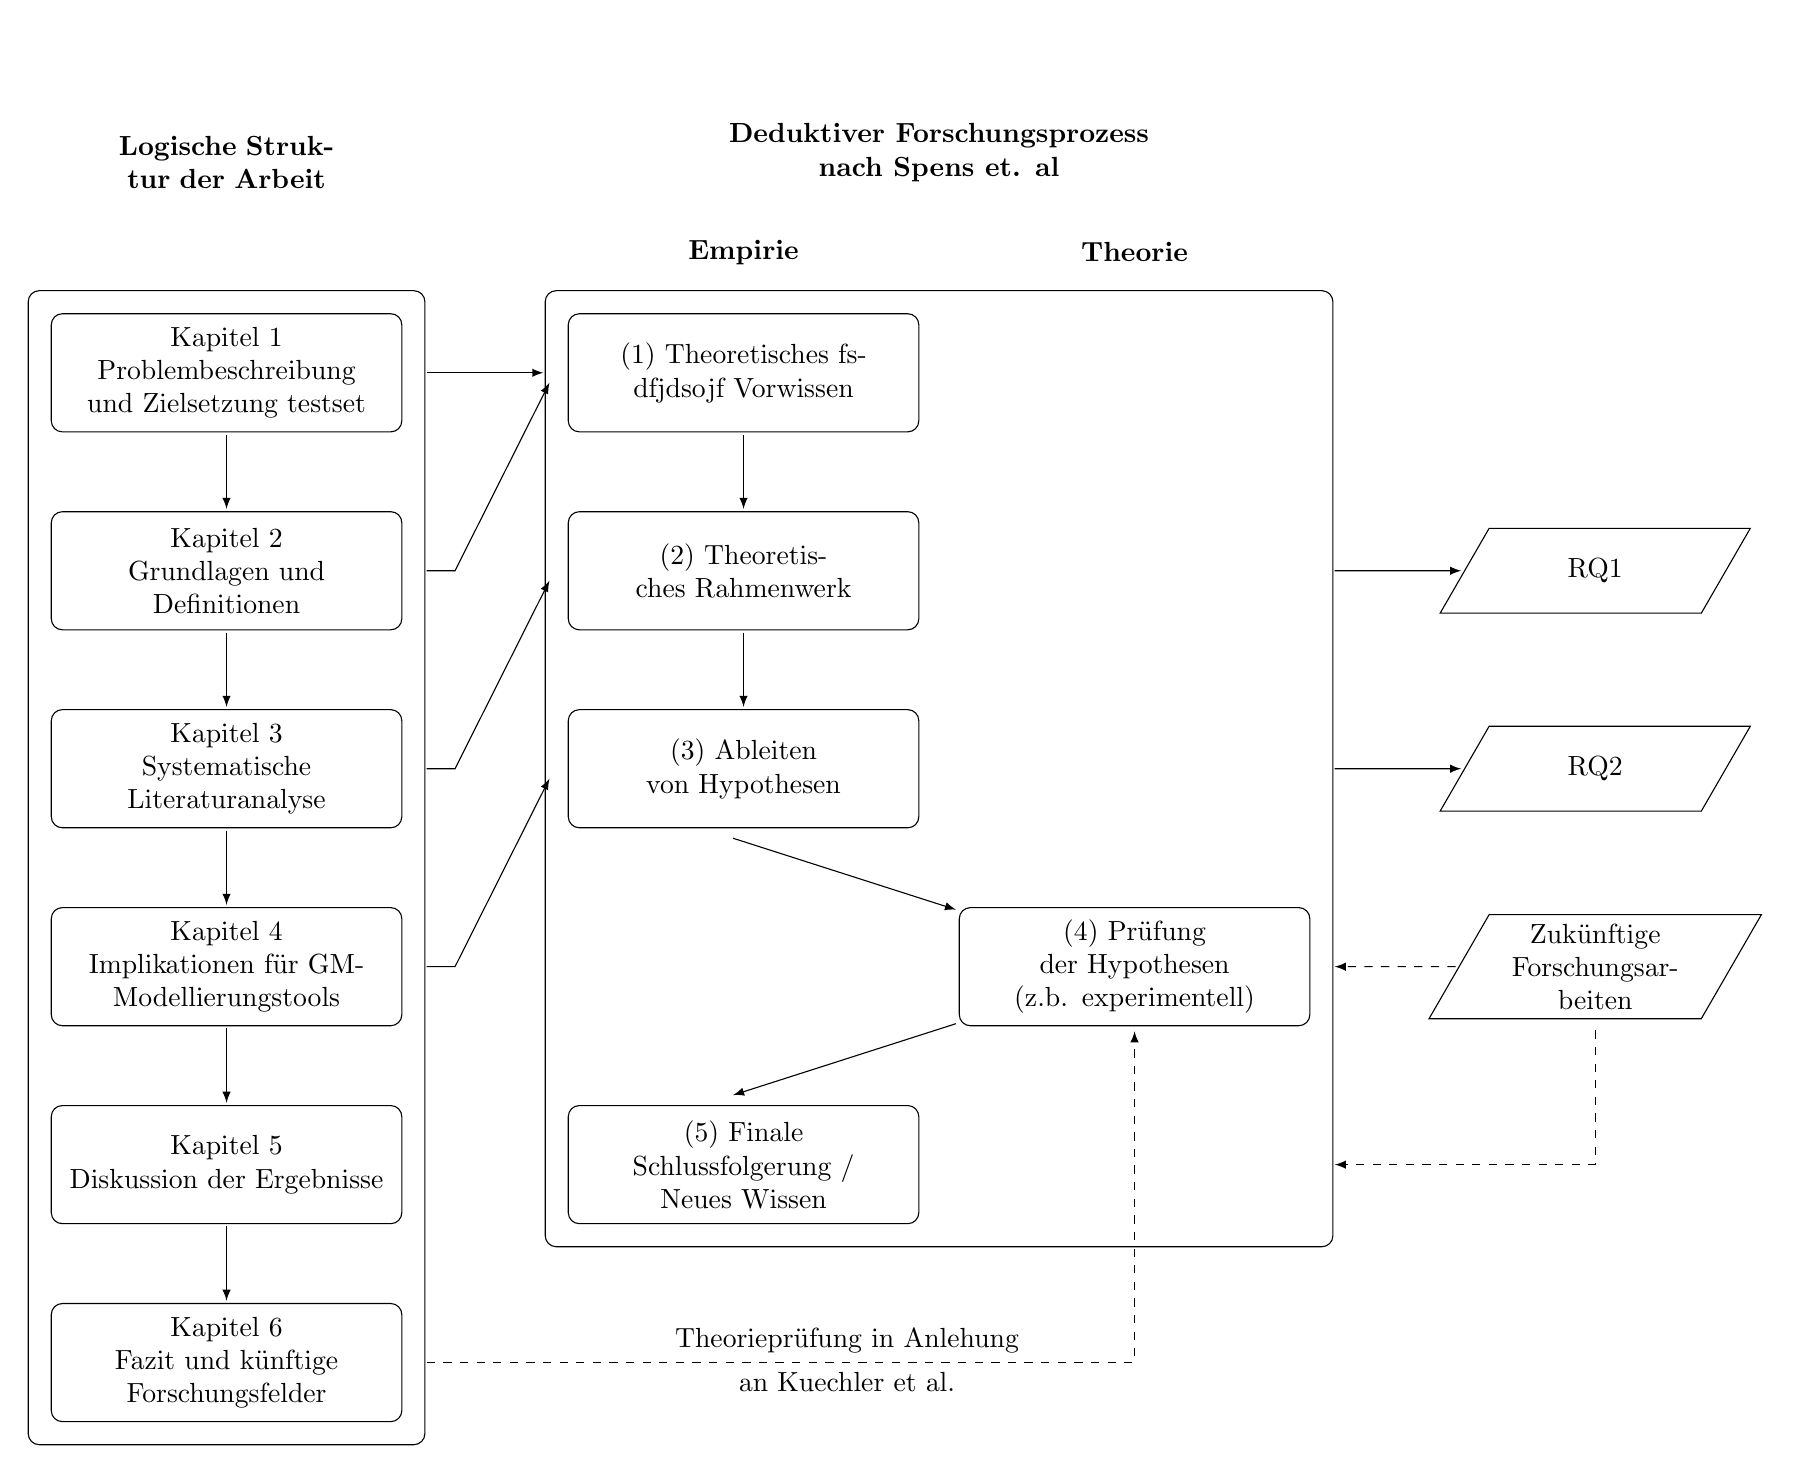
\begin{tikzpicture}
[auto, 
decision/.style={diamond, draw=blue, thick, fill=blue!20,text width=4.5em,align=flush center,inner sep=1pt},
block/.style ={ rectangle, draw, fill=white,  text centered, minimum height=15mm, text width=12em},
block_todo/.style ={ rectangle, draw, fill=white,  text centered, minimum height=15mm, text width=12em, rounded corners, outer sep=5},
block_done/.style ={ rectangle, draw, fill=white,  text centered, minimum height=15mm, text width=12em, rounded corners, outer sep=5},
block_normal/.style ={ rectangle, draw, fill=white,  text centered, minimum height=15mm, text width=12em, rounded corners, outer sep=5},
block_phantom/.style ={ block_normal, draw=none},
block_background/.style ={ rectangle,  draw=, fill=none,  text centered, minimum height=15mm,fill opacity=.1, rounded corners},
output/.style ={trapezium,draw,fill=none, minimum height=10mm,  align=center, trapezium left angle=60, trapezium right angle=120, text width=70},
line_inner/.style ={draw, -latex,shorten >=-4pt, shorten <=-4pt},
line_outer/.style ={draw, -latex,shorten >=4pt, shorten <=4pt}]
]


\matrix (table) [column sep=1.5cm,row sep=1cm, ampersand replacement=\&,  nodes in empty cells, in front of path]
{
% row 1
\node [block_normal, draw=none] (11) {\textbf{Logische Struktur der Arbeit}};\& [.6cm]
 \node [block_normal, fill=none, draw=none] (12) {\\ \quad\\\quad\\\quad\\\quad\\\quad\\\textbf{Empirie}}; \&[-1cm]
 \node [block_normal, fill=none, draw=none] (13) {\\ \quad\\\quad\\\quad\\\quad\\\quad\\\textbf{Theorie}};  \& [0cm]
 \node [] (14) {};   \\[-.5cm]

% row 2
\node [block_normal] (21) {Kapitel 1\\Problembeschreibung und Zielsetzung testset};
\&  \node [block_done] (22) {(1) Theoretisches fsdfjdsojf Vorwissen};
\&  \node [block_phantom] (23) {};
\&  \node [] (24) {};
\\

% row 3
\node [block_normal] (31) {Kapitel 2\\Grundlagen und Definitionen}; \& 
\node [block_done] (32) {(2) Theoretisches Rahmenwerk};  
\&\node [block_phantom] (33) {};  ;
\& \node [output] (34) {RQ1\vphantom{\begin{tabular}{c}x\\ y\end{tabular}}};
\\
% row 4
\node [block_normal] (41) {Kapitel 3\\Systematische Literaturanalyse}; \&
\node [block_done] (42) {(3) Ableiten von Hypothesen}; \&   
\node [block_phantom] (43) {}; 
 \&\node [output] (44) {RQ2\vphantom{\begin{tabular}{c}x\\ y\end{tabular}}};\\
 
% row 5
\node [block_normal] (51) {Kapitel 4\\Implikationen f\"ur GM-Modellierungstools}; \& 
\node [block_phantom] (52) {}; \&  
\node [block_done] (53) {(4) Pr\"ufung der Hypothesen\\ (z.b. experimentell)};
 \&\node [output] (54) {Zuk\"unftige Forschungsarbeiten}; \\

% row 6
\node [block_normal] (61) {Kapitel 5\\Diskussion der Ergebnisse};\& 
\node [block_done] (62) {(5) Finale Schlussfolgerung / \\Neues Wissen};
 \& \node [block_phantom] (63) {};
 \&  \node [] (64) {};\\
 
% row 7
\node [block_normal] (71) {Kapitel 6\\Fazit und k\"unftige Forschungsfelder}; \& 
\node [block, fill=none, draw=none] (72) {};  \&  
\node [block, fill=none, draw=none] (73) {};\&  
\node [] (74) {};\\
};


\begin{scope}[on background layer]
%%%HEADER%%%%%
\node[fit=(12)(13), draw=none, minimum height=1cm, fill=none]{\textbf{Deduktiver Forschungsprozess\\ nach Spens et. al}};
%%%%%SPALTE1%%%%%%%%%
\node[fit=(21)(71), block_background, fill=white]{};
%%%%%SPALTE2%%%%%%%%
\node[fit=(22)(63), block_background]{};
\end{scope}
 
 
%Pfeile Kapitelstruktur
 \draw [line_inner](21) to [bend left=0] node [above] {} (31)  ;
 \draw [line_inner](31) to [bend left=0] node [above] {} (41)  ;
 \draw [line_inner](41) to [bend left=0] node [above] {} (51)  ;
 \draw [line_inner](51) to [bend left=0] node [above] {} (61)  ;
 \draw [line_inner](61) to [bend left=0] node [above] {} (71)  ;


%Pfeile Prozess
 \draw [line_inner](22) to [bend left=0] node [above] {} (32);
 \draw [line_inner](32) to [bend left=0] node [above] {} (42)  ;
 \draw [line_inner](42.south) to [bend left=0] node [above] {} (53)  ;
 \draw [line_inner](53) to [bend left=0] node [above] {} (62.north)  ;

%Pfeile Interaktion Kapitel Prozess
 \draw [line_outer](21.east) to [bend left=0] node [above] {} (22.west)  ;
% \draw [line_outer](31.east) to [bend left=0] node [above] {$$} (22.west)  ;
  \draw [line_outer](31.east) -| ++ (.5,0) --  node [above] {} (22.west)  ;
% \draw [line_outer](41.east) to [bend left=0] node [above] {$$} (32.west)  ;
 \draw [line_outer](41.east) -| ++ (.5,0) --  node [above] {} (32.west)  ;
 %\draw [line_outer](51.east) to [bend left=0] node [above] {$$} (42.west)  ;
  \draw [line_outer](51.east) -| ++ (.5,0) --  node [above] {} (42.west)  ;
 %\draw [line](61) to [bend left=0] node [above] {$$} (22)  ;
% \draw [line](71.east) to [bend right=40] node [above] {$$} (53)  ;
 \draw [line_outer, dashed,shorten >=-3pt](71.east) -|   node [above, pos=.3] {Theoriepr\"ufung in Anlehung }  node [below, pos=.3] {an Kuechler et al.}(53)  ;
 
%Pfeile Output
 \draw [line_outer, shorten >=1pt](33) to [bend left=0] node [above] {} (34)  ;
 \draw [line_outer,shorten >=1pt](43) to [bend left=0] node [above] {} (44)  ;
 \draw [line_outer, dashed,shorten <=1pt](54) to [bend left=0] node [above] {} (53)  ;
  \draw [line_outer, dashed](54) |-  node [above] {} (63)  ;

\end{tikzpicture}%
}%
\end{document}%